The CI/CD process of most software projects can be broken down into these parts:

\begin{itemize}
    \item Version control
    \item Code Review
    \item Building
    \item Automated Testing
    \item Deployment
\end{itemize}

Hence, these points will be the dimensions of the tool-chain comparison.

\begin{figure}[h]
    \centering
    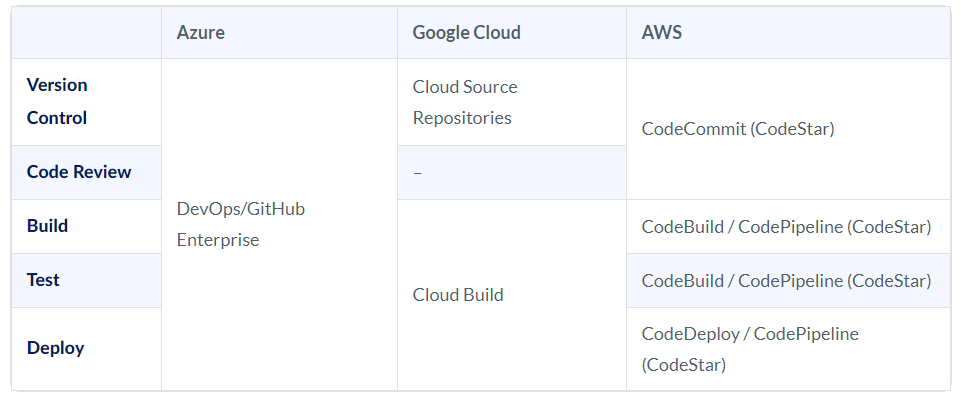
\includegraphics[width=16cm]{images/ToolChainCompare.png}
    \caption{Tool-Chain Comparison}
    \label{fig:ci-cd-pipeline-chain-compare}
\end{figure}

After analysing Figure-5, following set of deductive comparison could be made:\footnote{\url{https://www.inovex.de/en/cloud-native-cicd-part-2-azure-devops-vs-aws-vs-google-cloud/}}

\begin{itemize}
    \item \textbf{Service Comparison} -  Azure DevOps offers a complete service suite, a set of services that integrates seamlessly. There are sub-parts but everything is coherent and there is one tool for one job. Google is half-way there with a conjunction of two services. Whereas, AWS has more of a toolbox. It has a myriad of services that a user needs to find and combine in order to establish a secure pipeline. AWS presents a steeper learning curve to the new-comers, which can slow down the entire development process.
    \item \textbf{Version Control and Code Review} - Azure DevOps Repos workflow is exactly as same a GitHub Enterprise, which facilitates better code review capabilities. AWS CodeCommit supports pull request workflows like GitHub or GitLab but it’s just not as user-friendly and intuitive as them. Google Cloud Source Repositories are a remote git back-end in the most basic sense. It's possible to push and pull from it. Not more, not less. Code reviews on feature branches are rather important and not possible with GCP Cloud Source Repositories.
    \item \textbf{Build and Test} - For building and performing automated tests, Azure and AWS provides a myriad of options through their management console. It is possible to build an application regardless of its development language and integrated build tools like Gradle, Maven or Ant. However, in Google Cloud Build the service comes with a limited set of around 20 official cloud builder Docker images. These official images support most common tool chains. However, on top of those official images, there are community images for a lot more project (Terraform, Ansible, Android etc.) . GCP does not provide pre-built containers for those images. A developer has to clone the needed spec, build the image and push it to the container registry of the project before usage. 
    \item \textbf{Deployment} - In terms of deploying an application, all of the cloud platforms provide a range of options from server-less options to standard containerized web apps and more. However, Microsoft Azure trumps AWS and GCP in this category for one reason. Since Azure DevOps is a independent service suite, it is not limited to deploying applications to in-house solutions like Azure Portal. Azure DevOps can deploy an application in other cloud vendor portals like AWS Managemnt Console or GCP Platform or even to on-premise servers.
\end{itemize}

After analyzing all the core parts of the CD-CD process of all three cloud providers, Microsoft Azure DevOps seems the most viable option to implement a CI-CD pipeline in the cloud for the following reasons: 

\begin{itemize}
    \item Azure DevOps Repos are essentially the same as Github and GitHub Enterprise, since Microsoft acquired GitHub in 2018. Similar architecture and workflow as GitHub means a familiar environment for the developers which provides convenience and also can speed up development process.
    \item It provides IaaC support for almost all the popular tools such as Chef, Puppet, Ansible and Terraform through official images for configuring and provisioning development, QA and production environments. In other platforms like GCP, third-party images are needed to use those tools.
    \item There are less possibility of vendor lock-in in Azure DevOps. Because it can deploy applications to multiple cloud and on-premise solutions. Thus, if the need of vendor migration arises the process will be seamless. 
    \item Azure DevOps service is completely free for up-to 5 users. From 6 users and on-wards a small fee of 6 USD is charged on a bi-monthly basis per user. Unlike other cloud services like AWS and GCP, there are no cost for pipeline execution or storing application code in Repos. Application artifact storage is also free up-to 2 gigabyte. 
\end{itemize}
